%!TEX root = ../thesis.tex
%*******************************************************************************
%*********************************** First Chapter *****************************
%*******************************************************************************

\chapter{Introduction}  %Title of the First Chapter
\lhead{Chapter 1. \emph{Introduction}}


High-dimensional datasets, where the number of variables, $p$, is greater then the sample size, $n$, are increasingly becoming common in many feilds, particularly in genatics. For example, gene expresion dataset used by \cite{eisen1998cluster} has 2467 variables and 79 samples. Another study by \cite{tamayo1999interpreting} has 6817 variables (human genes) obtained from 72 microarray images. A relatively recent cancer study by \cite{beerenwinkel2007genetic} which is based on a dataset with 78 genes ($p$) and only 35 samples ($n$).

In these types of high-dimensional datasets, the sample covariance matrix\textemdash maximum likelihood estimator and its unbiased version\textemdash perform poorly and are not considered a good approximation to the true covariance matrix (even if $n$ is comparable to $p$). This is because the sample covariance matrix contains estimation error and their eigenvalues tends to be overdispersed; that is, the larger eigenvalues will contain a high amount of positive errors (overestimated) and smaller eigenvalues will contain a high amount of negative errors (underestimated). In addition, the inverse covariance matrix is fundamental to multivariate methods comprising regression, Gaussian graphical models, linear discriminant analysis and Mahalanobis distance. The sample covariance matrix loses its full rank and is not invertible if $p$ exceeds $n$. The non-invertibility of the sample covariance matrix renders the above mentioned multivariate methods inapplicable.  
 
To make things more clear, we conduct a small simulation study. We draw samples of size $n = \lbrace$25, 50, 100, 1000$\rbrace$ from a $p$-variate normal distribution with mean vector, $\pmb{\mu}=\textbf{0}$, and an identity covariance matrix, $\pmb{\Sigma} = \pmb{I}$. We fix the number of variables, $p=50$. For each value of $n$ we repeat the simulations 1000 times and the average estimated eigenvalues are portrayed in Figure \ref{Fig1.1}. It is clear from the Figure that, due to estimation error, the larger eigenvalues are overestimated and the smaller eigenvalues are underestimated. The estimation error decreases as we increase the sample size. Moreover, if the number of observations are less then the number of variables, the sample covariance matrix becomes singular and is not invertible (product of the eigenvalues become zero).
 
 To deal with high-dimensional covariance estimation problems, various methods have been proposed in the previous literature. In this Thesis, first we want to explore some of the well known shrinkage (regularization) methods. Further, these shrinkage methods rely on a tuning parameter whose value need to be chosen in a suitable range of values. An appropriate choice of the tuning parameter leads to improved estimate of the covariance matrix. Our second objective is to choose an appropriate value of the tuning parameter, which we achieve by maximizing a multivariate normal likelihood function. Third, we shrink the sample covariance matrix towards more informative target estimators rather than using identity matrix as a target estimator.   


\begin{figure}[h]
    	\begin{center}
    		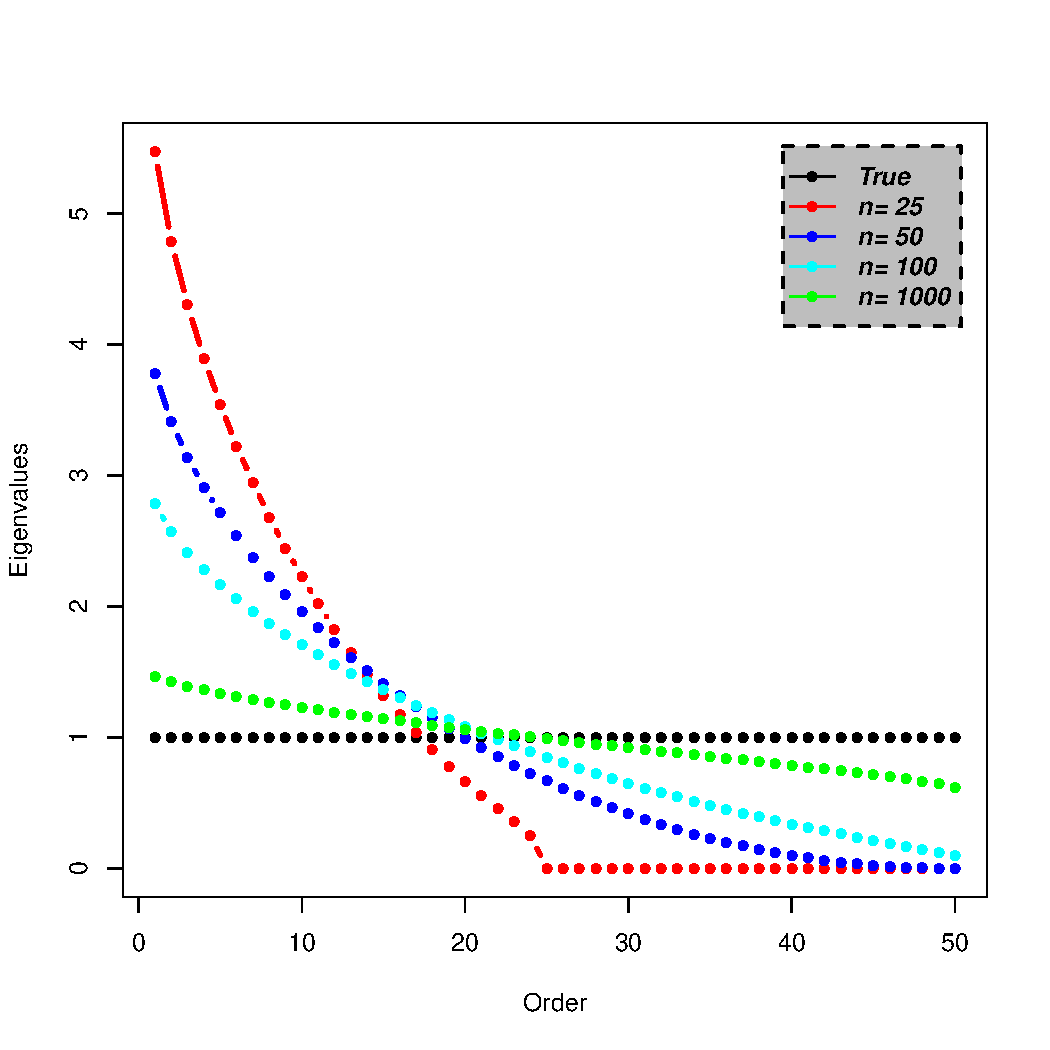
\includegraphics[scale=0.55]{screeplot.pdf}
    		\caption{Sorted eigenvalues of the true and sample covariance matrices for a fixed $p$=50 and $n = \lbrace$25, 50, 100, 1000$\rbrace$ drawn from multivariate normal distribution with Identity matrix as a true covariance matrix.} 
    		\label{Fig1.1}
    	\end{center}
    \end{figure}

